\documentclass[letterpaper]{article}
\author{Leon Bonde Larsen}
\title{Overview and considerations concerning data link layer}
\begin{document}
\setlength{\baselineskip}{1.6\baselineskip}
\setlength{\parskip}{2ex}
\maketitle

\section{Overview and considerations concerning data link layer}

\begin{figure}[htb]
	\begin{center}
	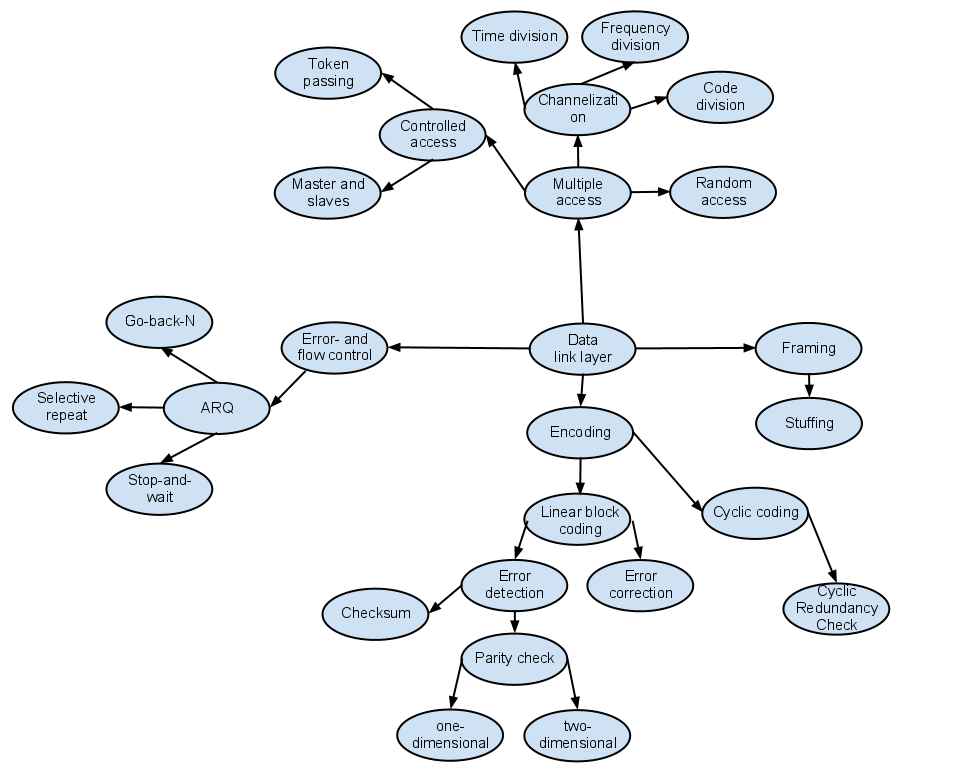
\includegraphics[scale=1,trim=0 0 0 0]{bobler_dll.png} %trim=l b r t (can cut off from every side)
	\caption{Things to consider concerning data link layer}
	\label{Things to consider concerning data link layer}			% figure labels are of the form \label{fig:*}
	\end{center}
\end{figure}

\subsection{Encoding}
First thing to consider is the encoding of signals. Since there are sixteen
different DTMF combinations, each tone can carry four bits.

The only type of error to consider is the situation where a tone is
misinterpreted, which leads to a four bit burst error. Therefore the system
should be designed specifically to detect errors of this type. Since the media
is considered to be very noisy, transmissions should also be kept as short as
possible.

A two dimensional parity check will be able to detect burst errors of the
proposed size, so this is the choice. Implementing the parity check as a
four-by-four matrix will make it possible to transfer two bytes with a frame of
three bytes.

Example: We want to transmit the two bytes 0011 0101 and 0101 1110. The data
link layer puts these in a four by four matrix and calculates the parity bits by
adding the rows and columns:


\begin{table}[htb]
	\begin{center}
	\begin{tabular}{c|c}
	0011 & 0 \\
	0101 & 0 \\
	0101 & 0 \\
	1110 & 1 \\
	\hline
	1101 & \\
	\end{tabular}
	\end{center}
	\caption{Two-dimensional parity check}
	\label{tab:Two-dimensional parity check}
\end{table}

Instead of as normally done to increase the size of each row by one to contain
the parity bit, the parity bits are transmitted together as a redundant byte. In
the case of this example the transmission would be:

\begin{table}[htb]
	\begin{center}
	\begin{tabular}{c|c|c|c|c|c}
	0011 & 0101 & 0101 & 1110 & 0001 & 1101 \\
	\end{tabular}
	\end{center}
	\caption{Bytes to be transmitted}
	\label{tab:Bytes to be transmitted}
\end{table}

Each four bit nipple is now transmitted an a DTMF-tone. Should one of the tones
be misinterpreted, the receiving data link layer would get a mismatch of the
parity bits for example:

\begin{table}[htb]
	\begin{center}
	\begin{tabular}{c|c}
	0011 & 0 \\
	0101 & 0 \\
	0000 & 0 \\
	1110 & 1 \\
	\hline
	1000 & \\
	\end{tabular}
	\end{center}
	\caption{Failed parity check}
	\label{tab:Failed parity check}
\end{table}


This will lead to the frame being discarded. Though in some cases it will be
possible to correct the error and find the original nibble, this is not
recommended, since more than one tone might be corrupted. Errors in the
redundant byte will also lead to the discarding of the transmission.


\subsection{Flowcontrol}
The next thing to consider is flowcontrol. Since the DTMF-system
cannot be used as full-duplex, piggybacking is impossible. This means that at
some point the receiver must reply. This reply will also be of six-tones, and
therefore it might as well contain information about witch frames to resend. In
other words a selective repeat system is preferred

To introduce a selective repeat system, additional redundancy is needed.

By using only two bits for the sequence number, redundancy is kept as low as
possible while still benefiting from pipelining. The sender transmits four
frames (twentyfour tones) and then waits for the receiver to reply with one frame (six
tones).

\subsection{Framing}
It is presumed that the physical layer will provide a starting point for each
transmission, probably in the form of silence. If this is not the case,
additional flags will be needed in between the frames, again leading to the need
of stuffing.

Next thing to consider is multipoint. There are three options: A token
network, a time division network or a code division network. Time division
requires a level of timing the interface layer is not able to deliver.
Code division leads to the need for larger frames or if implemented with the
proposed frame size, a lot of unused frames in a small network. This leaves us
with a token passing network, so this is the choice.

Four bits will control the adressing. The first two
bits identifies the receiver and the next two identifies the sender. Thereby the
protocol allows networks of up to four stations.

The selective repeat system and the token network introduces the need for different frame types.
The type field will consist of two bits, at the same time controlling
the token and indicating frame types. Rules must be implemented to keep the token circulating.

\begin{table}[htb]
	\begin{center}
	\begin{tabular}{|c|ll|}
		\hline
		00 & Has no token & Reply from receiver \\
		\hline
		01 & Has no token & Passes token to receiveradress \\
		\hline
		10 & Has token & Accepts token from receiveradress \\
		\hline
		11 & Has token & Data frame for receiveradress \\
		\hline
	\end{tabular}
	\end{center}
	\caption{Protocol for type field}
	\label{tab:Protocol for type field}
\end{table}

This leads to the following format of a frame: 

\begin{table}[htb]
	\begin{center}
	\begin{tabular}{|ccc|c|c|}
		\hline
		type (2 bits) & address (4 bits) & sequence (2 bits) & data (8 bits) & parity (8 bits)  \\
		\hline
	\end{tabular}
	\end{center}
	\caption{Final frame format}
	\label{tab:Final frame format}
\end{table}

\today

\end{document}